\chapter{Matematický model}
\label{kap:matematicky_model}
\section{Krivky druhého stupňa}
Nasledujúca teória a klasifikácia nadplôch druhého rádu je prevzatá zo \cite{Ivan}, \cite{Kor13}, \cite{Gla16}, \cite{Ode20}, \cite{Zla11}.
Krivka druhého stupňa $c$ je v karteziánskych súradniciach $(x, y) \in \mathbb{E}^2$ daná rovnicou 
$$ q(x, y) = Ax^2 + Bxy + Cy^2 + Dx + Ey + F = 0.$$
Prípad $A = B = C = 0$  môžeme vylúčiť, pretože potom je rovnica lineárna a opisuje priamku. Vo všeobecnosti rovnica vyjadruje kužeľosečku, ktorá je daná piatimi bodmi. Ak $F \neq 0$, môžeme ju vydeliť $F$ a potom riešiť sústavu lineárnych rovníc s piatimi neznámymi. Okrem klasických prípadov, ako elipsy, paraboly a hyperboly, môžu kužeľosečky degenerovať na dvojice priamok, bod alebo prázdnu množinu.

V algebraickom zmysle má kužeľosečka $c$ vždy dva priesečníky $S_1$ a $S_2$ s danou priamkou $s$. Oba môžu byť reálne alebo komplexne združené. Limitný prípad $S_1 = S_2$ nastáva vtedy, keď $s$ je dotyčnicou k $c$.

V závislosti od počtu reálnych priesečníkov s priamkou $s$ v nekonečne rozlišujeme tri typy kužeľosečiek 
\begin{enumerate}
\item eliptický typ: bez reálnych priesečníkov,
\item hyperbolický typ: dva reálne priesečníky,
\item parabolický typ: priamka v nekonečne sa dotýka krivky.
\end{enumerate}

Matica $A \in \mathbb{R}^{n \times n}$ sa nazýva ortogonálna, ak platí $A^T \cdot A = I_n$, alebo, čo je to isté, $A^{-1} = A^T$. Prvá podmienka hovorí, že stĺpce matice $A$ tvoria ortonormálnu bázu euklidovského priestoru $\mathbb{R}^n$ so štandardným skalárnym súčinom. Potom tiež platí $A \cdot A^T = I_n$, teda takisto riadky matice $A$ tvoria ortonormálnu bázu v $\mathbb{R}^n$. 

\begin{theorem} 
Matica prechodu od ortonormálnej bázy v $\mathbb{R}^n$ so štandardným skalárnym súčinom k ortonormálnej báze je ortogonálna matica. Tiež, ak od ortonormálnej bázy v $\mathbb{R}^n$ prejdeme pomocou ortogonálnej matice prechodu k novej báze,
tak aj nová báza bude ortonormálna.
\end{theorem}

\subsection{Invarianty kriviek druhého stupňa}
\begin{definition}
Invariantom krivky druhého stupňa, vyjadrenej rovnicou
$$
q(x, y) = a_{11}x^2 + 2a_{12}xy + a_{22}y^2 + 2a_{13}x + 2a_{23}y + a_{33} = 0
$$
je každý taký algebraický výraz, závisiaci od \(a_{11}, a_{12}, a_{22}, a_{13}, a_{23}, a_{33}\), ktorého hodnota sa nezmení, ak túto krivku vyjadríme v inom karteziánskom súradnicovom systéme, ku ktorému prejdeme pomocou otočení alebo posunutí (čím od rovnice, viažúcej staré premenné \(x, y\), prejdeme k rovnici, viažúcej nové premenné \(x', y'\)).
\end{definition}

\begin{theorem}
Nasledujúce číselné výrazy sú invariantmi krivky druhého stupňa, vyjadrenej rovnicou $q(x, y)$.
\begin{align*}
\Delta(x,y) &= \det \begin{pmatrix} 
a_{11} & a_{12} & a_{13} \\ 
a_{12} & a_{22} & a_{23} \\
a_{13} & a_{23} & a_{33} \end{pmatrix}, \
\delta(x,y) = \det \begin{pmatrix} a_{11} & a_{12} \\ a_{12} & a_{22} \end{pmatrix}, \
s(x,y) &= a_{11} + a_{22}.
\end{align*}
\end{theorem}
Z tohto možno odvodiť nasledujúcu klasifikáciu kužeľosečiek.

%\begin{table}[h]
%\centering
%\begin{tabular}{|c|c|c|l|}
%\hline
%\textbf{Typ} & $\delta$ & $\Delta$ & \textbf{Tvar}  \\
%\hline
%\multirow{3}{*}{eliptický} & \multirow{3}{*}{$> 0$} & $\neq 0$ & ak $s\Delta < 0$, tak elipsa \\
%& & $\neq 0$ & ak $s\Delta > 0$, tak  $\emptyset$ \\
%& & $= 0$ & bod \\
%\hline
%\multirow{2}{*}{hyperbolický} & \multirow{2}{*}{$< 0$} & $\neq0$ & hyperbola \\
% & & $=0$ & dve rôznobežné priamky \\
%\hline
%\multirow{4}{*}{parabolický} & \multirow{4}{*}{$= 0$} & $\neq0$ & parabola \\
%& & $=0$ & dve rovnobežné priamky \\
%& & $= 0$ & priamka \\
%& & $= 0$ & $\emptyset$ \\
%\hline
%\end{tabular}
%\caption{Klasifikácia kužeľosečiek.}
%\label{tab:conic_sections}
%\end{table}

\begin{table}[h]
\centering
\begin{tabular}{|l|l|l|l|}
\hline
\textbf{Typ} & $\delta$ & $\Delta \neq  0$ & $\Delta = 0 $ \\
\hline
\multirow{2}{*}{eliptický} & \multirow{2}{*}{$> 0$} & ak $s\Delta < 0$, tak elipsa & \multirow{2}{*}{bod} \\
& & ak $s\Delta > 0$, tak $\emptyset$ & \\
\hline
hyperbolický & $< 0$ & hyperbola & dve rôznobežné priamky \\
\hline
\multirow{3}{*}{parabolický} & \multirow{3}{*}{$= 0$} & dve rovnobežné priamky & \multirow{3}{*}{parabola} \\
& & priamka & \\
& & $\emptyset$ & \\
\hline
\end{tabular}
\caption{Klasifikácia kužeľosečiek.}
\label{tab:conic_sections}
\end{table}

\section{Plochy druhého stupňa}
Plocha druhého stupňa $Q$ je v karteziánskych súradniciach $(x, y, z) \in \mathbb{E}^3$ daná rovnicou
\[ q(x, y, z) = Ax^2 + By^2 + Cz^2 + Dxy + Exz + Fyz + Gx + Hy + Iz + J = 0. \]
Je zrejmé, že ak je prvých šesť koeficientov nulových, uvedená rovnica je lineárna a opisuje rovinu v priestore. Vo všeobecnosti rovnica opisuje kvadriku, ktorá je daná deviatimi bodmi. Ak $J \neq 0$, môžeme ju vydeliť $J$ a potom vyriešiť sústavu lineárnych rovníc s deviatimi neznámymi. Okrem klasických prípadov, ako elipsoidy, paraboloidy a hyperboloidy, môžu kvadriky degenerovať aj na kvadratické kužele, kvadratické valce a dvojice rovín.

V algebraickom zmysle je kvadrika $Q$ plocha druhého stupňa, ktorá má vždy dva priesečníky $S1$ a $S2$ s danou priamkou $s$. Oba môžu byť reálne alebo komplexne združené. Limitný prípad $S1 = S2$ nastáva vtedy, keď $s$ je dotyčnicou $Q$.

V závislosti od počtu reálnych priesečníkov s rovinou $s$ v nekonečne rozlišujeme tri typy kvadrík:
\begin{enumerate}
\item eliptický typ: bez reálnych priesečníkov,
\item hyperbolický typ: dva reálne priesečníky,
\item parabolický typ: kvadriky sa dotýka rovina v nekonečne.
\end{enumerate}

Nasledujúce číselné výrazy sú invariantmi plochy druhého rádu, vyjadrenej rovnicou 
\[ q(x, y, z) = a_{11}x^2 + a_{22}y^2 + a_{33}z^2 + 2a_{12}xy + 2a_{13}xz + 2a_{23}yz + 2a_{14}x + 2a_{24}y + 2a_{23}z + a_{44} = 0. \]
\begin{align*}
\Delta(x, y, z) &= \det \begin{pmatrix} 
a_{11} & a_{12} & a_{13} & a_{14} \\ 
a_{21} & a_{22} & a_{23} & a_{24} \\
a_{31} & a_{32} & a_{33} & a_{34} \\
a_{41} & a_{42} & a_{43} & a_{44}
\end{pmatrix}, \
\delta(x, y, z) = \det \begin{pmatrix} 
a_{11} & a_{12} & a_{13} \\ 
a_{21} & a_{22} & a_{23} \\ 
a_{31} & a_{32} & a_{33} 
\end{pmatrix}
\end{align*}
\begin{align*}
T(x, y, z) &= \det \begin{pmatrix} 
a_{11} & a_{12} \\ 
a_{21} & a_{22} 
\end{pmatrix} + \det \begin{pmatrix} 
a_{22} & a_{23} \\ 
a_{32} & a_{33} 
\end{pmatrix} + \det \begin{pmatrix} 
a_{33} & a_{31} \\ 
a_{13} & a_{11} 
\end{pmatrix}, 
\end{align*}
\begin{align*}
s(x, y, z) &= a_{11} + a_{22} + a_{33}, \ \Delta'(x, y, z) = \Delta_{11} + \Delta_{22} + \Delta_{33}, 
\end{align*}
kde $
\Delta_{ij} = (-1)^{i+j} \det(\Delta_{ij}).$

Z tohto možno odvodiť nasledujúce dve tabuľky.

\begin{table}[h]
\centering
\begin{tabular}{|c|c|c|p{2.2cm}|p{2.15cm}|p{2cm}|}
\hline
Typ & $\delta$ & $s\delta$ a $T$ & $\Delta > 0$ & $\Delta < 0$ & $\Delta = 0$ \\
\hline
eliptický & $\neq 0$ & $s\delta>0$ a $T>0$ & $\emptyset$ & elipsoid & $\emptyset$ \\
\hline
hyperbolický & $\neq 0$ & $s\delta>0$ alebo $T \leq0$ & jednodielny hyperboloid & dvojdielny hyperboloid & kužeľ \\
\hline
parabolický & $=0$ & & hyperbolický paraboloid & eliptický paraboloid & valcové a reducibilné plochy \\
\hline
\end{tabular}
\caption{Klasifikácia kvadrík.}
\label{tab:classification_of_quadrics}
\end{table}

%\begin{table}[h]
%\begin{adjustbox}{center}
%\centering
%\begin{tabular}{|c|c|c|p{2.2cm}|p{2.15cm}|p{2cm}|}
%\hline
%Typ & $\delta$ & $s\delta$ a $T$ & $\Delta > 0$ & $\Delta < 0$ & $\Delta = 0$ \\
%\hline
%eliptický & $\neq 0$ & $s\delta>0$ a $T>0$ & $\emptyset$ & elipsoid & $\emptyset$ \\
%\hline
%hyperbolický & $\neq 0$ & $s\delta>0$ alebo $T \leq0$ & jednodielny hyperboloid & dvojdielny hyperboloid & kužeľ \\
%\hline
%parabolický & $=0$ & & hyperbolický paraboloid & eliptický paraboloid & valcové a reducibilné plochy \\
%\hline
%\end{tabular}
%\end{adjustbox}
%\caption{Klasifikácia kvadrík.}
%\label{tab:classification_of_quadrics}
%\end{table}

\begin{table}[h]
\centering
\begin{tabular}{|l|l|l|l|}
\hline
Typ & $T$ & $\Delta' \neq  0$ & $\Delta' = 0 $ \\
\hline
\multirow{2}{*}{eliptický} & \multirow{2}{*}{$> 0$} & ak $s\Delta < 0$, tak eliptický valec & \multirow{2}{*}{bod} \\
& & ak $s\Delta > 0$, tak $\emptyset$ &\\
\hline
hyperbolický & $< 0$ & hyperbolický valec & dve rôznobežné roviny \\
\hline
\multirow{3}{*}{parabolický} & \multirow{3}{*}{$= 0$} & \multirow{3}{*}{parabolický valec} & dve rovnobežné roviny \\
& & & rovina \\
& & & $\emptyset$ \\
\hline
\end{tabular}
\caption{Klasifikácia degenerovaných kvadrík.}
\label{tab:degenerate_quadrics}
\end{table}

\section{Obálka elíps}
\subsection{Zmena bázy}
Nech $m(t) \colon  I \subseteq \mathbb{R} \rightarrow \mathbb{R}^2$ je aspoň dvakrát diferencovateľná krivka, napíšme rovnicu elipsy $Q$ so stredom na krivke $m(t)$, hlavnou polosou $a$ v smere vektora $\dot{m}(t)$ a vedľajšou polosou $b$ v smere normálového vektora $n(t)$ ku krivke $m(t)$. Vydelením normou vektorov $\dot{m}(t)$ a $n(t)$ dostávame novú ortonormálnu bázu tvorenú stĺpcovými vektormi matice $P(t),$ kde
$$
P(t) = \frac{1}{ \| \dot{m}(t) \|} \left(\begin{matrix}
   \dot{m}_1(t) & n_1(t) \\
   \dot{m}_2(t) & n_2(t)
\end{matrix} \right).
$$
Keďže sme prešli od štandardnej bázy k ortonormálnej báze, matica $P(t)$ je ortogonálna, a teda
$$
P^{-1} = P^{T} = \frac{1}{ \| \dot{m}(t) \|} \left(\begin{matrix}
  \dot{m}_1(t) & \dot{m}_2(t) \\
    n_1(t) & n_2(t)
\end{matrix}\right).
$$
V súradniciach $(u(t), v(t))$ má elipsa $Q$ rovnicu v kanonickom tvare 
\begin{align*}
\frac{u^2(t)}{a^2} + \frac{v^2(t)}{b^2} = 1,
\end{align*}
kde vzťah medzi súradnicami $(u(t), v(t))$ a $(x,y)$ je daný
$$
\left(\begin{matrix}
u(t) \\
v(t)
\end{matrix}\right) = \frac{1}{ \| \dot{m}(t) \|}
\left(\begin{matrix}
  \dot{m}_1(t) & \dot{m}_2(t) \\
    n_1(t) & n_2(t)
\end{matrix}\right)
\left(\begin{matrix} \left(\begin{matrix} x \\ y \end{matrix}\right) - \left(\begin{matrix} m_1(t) \\ m_2(t) \end{matrix}\right) \end{matrix}\right).
$$
%\begin{equation*}
%\frac{{(x - m_1(t))^2}}{a_0^2} + \frac{{(y - m_2(t))^2}}{b_0^2} = 1
%\end{equation*}
%Matica prechodu k novej báze je tvaru
%$$
%A(t) = \left(\begin{matrix} \vec{t}(t) \quad \vec{n}(t)
%\end{matrix} \right),
%$$
%čo po rozpísaní do súradníc $\vec{t}(t) = \frac{1}{ \| \dot{m}(t) \|}( \dot{m}_1(t),  \dot{m}_2(t))$ a $\vec{n}(t) = \frac{1}{ \| \dot{m}(t) \|}( -\dot{m}_2(t),  \dot{m}_1(t))$ dáva 
%$$
%A(t) = \frac{1}{ \| \dot{m}(t) \|} \left(\begin{matrix}
%   \dot{m}_1(t) & n_1(t) \\
%   \dot{m}_2(t) & n_2(t)
%\end{matrix} \right).
%$$
%Keďže sme maticu $A(t)$ zostrojili tak, aby bola ortogonálna, ľahko dostávame aj vyjadrenie inverznej matice
%$$
%A^{-1}(t) = A^{T}(t) = \frac{1}{ \| \dot{m}(t) \|} \left(\begin{matrix}
%  \dot{m}_1(t) & \dot{m}_2(t) \\
%    n_1(t) & n_2(t)
%\end{matrix}\right).
%$$
%Vyjadrime elipsu $Q$ v novej báze $ u, v$ nasledovnou transformáciou
%
%kde 
%$$
%\left(\begin{matrix}
%u(t) \\
%v(t)
%\end{matrix}\right) = \frac{1}{ \| \dot{m}(t) \|}
%\left(\begin{matrix}
%  \dot{m}_1(t) & \dot{m}_2(t) \\
%    n_1(t) & n_2(t)
%\end{matrix}\right)
%\left(\begin{matrix}
%x-m_1(t) \\
%y-m_2(t) \\
%\end{matrix}\right).
%$$
Elipsa $Q$ sa potom transformuje na tvar
\begin{align} 
\label{eq:elipsa_v_novej_baze}
&\frac{1}{\|{\dot{m}}\|^2} \left( (x - m_1)^2 \left( \frac{{\dot{m}_1}^2}{a^2} + \frac{{\dot{m}_2}^2}{b^2} \right) + (y - m_2)^2 \left( \frac{{\dot{m}_2}^2}{a^2} + \frac{{\dot{m}_1}^2}{b^2} \right) \right) \\
+ &\frac{1}{\|{\dot{m}}\|^2} \left( 2\left( \frac{1}{a^2} - \frac{1}{b^2} \right)(x - m_1)(y - m_2)\dot{m}_1\dot{m}_2 \right) - 1 = 0,
\end{align}
po miernej úprave tak dostávame výraz
\begin{align*} 
&\frac{1}{a^2b^2\|\dot{m}\|^2} \left( (x - m_1)^2 \left( b^2 \dot{m}_1^2 + a^2 \dot{m}_2^2 \right) + (y - m_2)^2 \left( a^2 \dot{m}_1^2 + b^2 \dot{m}_2^2 \right) \right) \\
+ &\frac{1}{a^2b^2\|\dot{m}\|^2} \left( 2(b^2 - a^2)(x - m_1)(y - m_2)\dot{m}_1\dot{m}_2 \right) - 1 = 0.
\end{align*}
Uvažovali sme $\vec{n}=(-\dot{m}_2, \dot{m}_1), $ no výber orientácie normály nemá na výsledok žiaden vplyv.

\begin{example}[Parabola]
Majme parabolu s parametrizáciou $m(t)=(t, t^2), $ kde $\dot{m}(t)=(1, 2t).$ Transformujme elipsu,
\begin{align*}
&\frac{1}{a^{2} b^{2}\left(4 t^{2} + 1\right)} \left( (x-t)^2 (b^2 + a^{2} 4t^2) + (y-t^2)^2 (a^2 + b^2 4t^2) \right)\\
+ &\frac{1}{a^{2} b^{2}\left(4 t^{2} + 1\right)} \left( 2(b^2 - a^2)(x-t)(y-t^2)2t \right) - 1 = 0.
\end{align*}
\end{example}

\subsection{Výpočet obálky elíps}
Prepíšme rovnicu \ref{eq:elipsa_v_novej_baze} do maticového zápisu. Máme kužeľosečku $Q$ tvaru $$
Ax^2 + Bxy + Cy^2 + Dx + Ey + F = 0,$$
ktorá má v maticovom tvare vyjadrenie $X^TM(t)X = 0,$ kde $X=(x, y, 1) \in \mathbb{R}^3$ a $M(t)$ je symetrická matica rozmerov $3 \times 3$ s prvkami $A(t). \dots, F(t) $.
$$
\left(\begin{matrix} x \\ y \\ 1 
\end{matrix} \right)^T \left(\begin{matrix} 
A & \frac{B}{2} & \frac{D}{2} \\
\frac{B}{2} & C & \frac{E}{2} \\
\frac{D}{2} & \frac{E}{2} & F 
\end{matrix} \right)\left(\begin{matrix} x \\ y \\ 1 
\end{matrix} \right) = 0.
$$
Koeficienty matice $M(t)$ majú nasledovný tvar
\begin{align*}
A &= \frac{b^2 \dot{m}_1^2 + a^2 \dot{m}_2^2}{a^2b^2 \| \dot{m} \|^2} \\
B &= \frac{2(b^2-a^2)\dot{m}_1 \dot{m}_2}{a^2b^2 \| \dot{m} \|^2} \\
C &= \frac{a^2 \dot{m}_1^2 + b^2 \dot{m}_2^2}{a^2b^2\| \dot{m} \|^2} \\
D &= \frac{- 2m_1 \left( b^2 \dot{m}_1^2 + a^2 \dot{m}_2^2 \right) - 2 \left(b^2 - a^2 \right) m_2 \dot{m}_1 \dot{m}_2 }{a^2b^2\| \dot{m} \|^2} \\
E &= \frac{- 2m_2 \left( a^2 \dot{m}_1^2 + b^2 \dot{m}_2^2 \right) - 2 \left(b^2 - a^2 \right) m_1 \dot{m}_1 \dot{m}_2 }{a^2b^2\| \dot{m} \|^2} \\
F &= \frac{\dot{m}_1^2 (b^2 m_1^2 + a^2 m_2^2 - a^2b^2) + 2 (b^2 - a^2) m_1 m_2 \dot{m}_1 \dot{m}_2 + \dot{m}_2^2 (a^2 m_1^2 + b^2 m_2^2 - a^2b^2) }{a^2b^2\| \dot{m}  \|^2}  -  1  \\
\end{align*}
Pozrime sa deriváciu jednoparametrického systému elíps podľa parametra $t.$ 
$$ \frac{\partial X^TM(t)X}{\partial t} \colon = X^T M(t)X.
$$
Máme teda kužeľosečku $\dot{Q}$ tvaru 
$$
\dot{A}x^2 + \dot{B}xy + \dot{C}y^2 + \dot{D}x + \dot{E}y + \dot{F} = 0$$
kde $\dot{A}(t), \dots, \dot{F}(t)$ sú prvky matice $\dot{M}(t).$
$$
\left(\begin{matrix} x \\ y \\ 1 
\end{matrix} \right)^T \left(\begin{matrix} 
A & \frac{B}{2} & \frac{D}{2} \\
\frac{B}{2} & C & \frac{E}{2} \\
\frac{D}{2} & \frac{E}{2} & F 
\end{matrix} \right)\left(\begin{matrix} x \\ y \\ 1 
\end{matrix} \right) = 0.
$$
\begin{align*}
\dot{A} &= \frac{2 ( b^2 - a^{2}) ( \ddot{m}_{1} \dot{m}_{2} - \dot{m}_{1} \ddot{m}_{2}) \dot{m}_{1} \dot{m}_{2}}{a^{2} b^{2} \|\dot{m} \|^4} \\
\dfrac{\dot{B}}{2} &= \frac{(a^{2} - b^{2}) (2 (\dot{m}_{1} \ddot{m}_{1} + \dot{m}_{2} \ddot{m}_{2}) \dot{m}_{1} \dot{m}_{2} - (\dot{m}_{1} \ddot{m}_{2} + \ddot{m}_{1} \dot{m}_{2}) \|\dot{m} \|^2)}{a^{2} b^{2} \|\dot{m} \|^2} \\
\dot{C} &= \frac{2 (b^2 - a^{2}) ( \dot{m}_{1} \ddot{m}_{2} - \ddot{m}_{1} \dot{m}_{2}) \dot{m}_{1} \dot{m}_{2}}{a^{2} b^{2} \|\dot{m} \|^2} \\
\end{align*}
\begin{align*}
\dfrac{\dot{D}}{2} &= \frac{ (2 a^{2} (m_{1} \dot{m}_{2} - m_{2} \dot{m}_{1}) (\dot{m}_{1} \ddot{m}_{1} + \dot{m}_{2} \ddot{m}_{2}) \dot{m}_{2} }{a^2b^2 \|\dot{m} \|^4} \\
&+ \frac{a^{2} (\| \dot{m} \|^2 (- 2 m_{1} \dot{m}_{2} \ddot{m}_{2} + m_{2} \dot{m}_{1} \ddot{m}_{2} + m_{2} \ddot{m}_{1} \dot{m}_{2})}{a^2b^2 \|\dot{m} \|^4} \\
&+\frac{b^{2} (m_{1} \dot{m}_{1} + m_{2} \dot{m}_{2}) (\dot{m}_{1} \ddot{m}_{1} + \dot{m}_{2} \ddot{m}_{2}) \dot{m}_{1}}{a^2b^2 \|\dot{m} \|^4} \\
&-\frac{b^{2} \| \dot{m} \|^2   (2 m_{1} \dot{m}_{1} \ddot{m}_{1} + m_{2} \dot{m}_{1} \ddot{m}_{2} + m_{2} \ddot{m}_{1} \dot{m}_{2} + (\dot{m}_{1})^{3} + \dot{m}_{1} (\dot{m}_{2})^{2}))}{a^2b^2 \|\dot{m} \|^4} \\
\dot{E} &= \frac{2 \cdot (2 a^{2} (- m_{1} \dot{m}_{2} + m_{2} \dot{m}_{1}) (\dot{m}_{1} \ddot{m}_{1} + \dot{m}_{2} \ddot{m}_{2}) \dot{m}_{1} + a^{2} (\| m \|^2 (m_{1} \dot{m}_{1} \ddot{m}_{2} + m_{1} \ddot{m}_{1} \dot{m}_{2} - 2 m_{2} \dot{m}_{1} \ddot{m}_{1}) + 2 b^{2} (m_{1} \dot{m}_{1} + m_{2} \dot{m}_{2}) (\dot{m}_{1} \ddot{m}_{1} + \dot{m}_{2} \ddot{m}_{2}) \dot{m}_{2} - b^{2} ((\dot{m}_{1})^{2} + (\dot{m}_{2})^{2}) (m_{1} \dot{m}_{1} \ddot{m}_{2} + m_{1} \ddot{m}_{1} \dot{m}_{2} + 2 m_{2} \dot{m}_{2} \ddot{m}_{2} + (\dot{m}_{1})^{2} \dot{m}_{2} + (\dot{m}_{2})^{3}))}{a^2b^2 \| \dot{m} \|^4} \\
\dot{F} &= \frac{2 (a^{2} (\dot{m}_{1} \ddot{m}_{1} + \dot{m}_{2} \ddot{m}_{2}) (- m_{1}^{2} (\dot{m}_{2})^{2} + 2 m_{1} m_{2} \dot{m}_{1} \dot{m}_{2} - m_{2}^{2} (\dot{m}_{1})^{2}) + a^{2} \| m \|^4 (m_{1}^{2} \dot{m}_{2} \ddot{m}_{2} - m_{1} m_{2} \dot{m}_{1} \ddot{m}_{2} - m_{1} m_{2} \ddot{m}_{1} \dot{m}_{2} + m_{2}^{2} \dot{m}_{1} \ddot{m}_{1}) - b^{2} (\dot{m}_{1} \ddot{m}_{1} + \dot{m}_{2} \ddot{m}_{2}) (m_{1}^{2} (\dot{m}_{1})^{2} + 2 m_{1} m_{2} \dot{m}_{1} \dot{m}_{2} + m_{2}^{2} (\dot{m}_{2})^{2}) + b^{2} ((\dot{m}_{1})^{2} + (\dot{m}_{2})^{2}) (m_{1}^{2} \dot{m}_{1} \ddot{m}_{1} + m_{1} m_{2} \dot{m}_{1} \ddot{m}_{2} + m_{1} m_{2} \ddot{m}_{1} \dot{m}_{2} + m_{1} (\dot{m}_{1})^{3} + m_{1} \dot{m}_{1} (\dot{m}_{2})^{2} + m_{2}^{2} \dot{m}_{2} \ddot{m}_{2} + m_{2} (\dot{m}_{1})^{2} \dot{m}_{2} + m_{2} (\dot{m}_{2})^{3}))}{a^2b^2 \| \dot{m} \|^4}  
\end{align*}
Determinant matice $\dot{M}(t) = 0, $ pre všetky $t$, čo znamená, že kužeľosečka je singulárna.
Pozrime sa na subdeterminant
$$
\dot{M}_{33}(t) = \dot{A} \dot{C} - \frac{\dot{B}^2}{4} =  -\frac{(b^2 - a^2)^2}{a^4b^4} \frac{ (\dot{m_1}\ddot{m_2} - \ddot{m_1}\dot{m_2})^2 + \dot{m_1}\dot{m_2}\ddot{m_1}\ddot{m_2}}{\|m\|^4}.
$$ 
Hodnota $\dot{M}_33(t) < 0, $ pre všetky $t,$ teda kužeľosečka degeneruje na dve rôznobežné priamky.

\section{Obálka elipsoidov}
Pre jednoparametrické systémy plôch druhého rádu existuje maticový zápis tvaru 
$$
S: X^TM(t)X = 0,
$$
kde $ X = (x, y, z)^T \in \mathbb{R}^3 $ a $M(t) $ je symetrická matica rozmeru $4x4, $ ktorej koeficienty sú závislé od $t \in I$.
Rovnicu jednoparametrického systému sfér $S$
$$ x^2 +y^2 +z^2 -2xm_1 -2ym_2 - 2zm_3 + m_1^2 + m_2^2 + m_3^2 - r^2 =0
,$$
tak vieme zapísať ako
$$
\left(\begin{matrix} x \\ y \\ z  \\ 1
\end{matrix} \right)^T \left(\begin{matrix} 
1 & 0 & 0 & - m_1 \\
0 & 1 & 0 & - m_2 \\
0 & 0 & 1 & - m_3 \\
- m_1 & - m_2 & - m_3 &  m_1^2 + m_2^2 + m_3^2 - r^2 \\
\end{matrix} \right)\left(\begin{matrix} x \\ y \\ z \\ 1
\end{matrix} \right) = 0. 
$$
Deriváciu jednoparametrického systému sfér $\dot{S}$
$$
-2x\dot{m}_1 -2y\dot{m}_2 - 2z\dot{m}_3 + 2m_1\dot{m_1} + 2m_2\dot{m_2} + 2m_3\dot{m_3} - 2r\dot{r} = 0
$$
možno tiež zapísať v tvare  $X^T\dot{M}(t)X = 0,$
kde $\dot{M}(t)= \dfrac{\partial M(t)}{\partial t}.$
$$
\left(\begin{matrix} x \\ y \\ z  \\ 1
\end{matrix} \right)^T \left(\begin{matrix} 
0 & 0 & 0 & - \dot{m}_1 \\
0 & 0 & 0 & - \dot{m}_2 \\
0 & 0 & 0 & - \dot{m}_3 \\
- \dot{m}_1 & - \dot{m}_2 & - \dot{m}_3 &  2m_1\dot{m_1} + 2m_2\dot{m_2} + 2m_3\dot{m_3} - 2r\dot{r} \\
\end{matrix} \right)\left(\begin{matrix} x \\ y \\ z \\ 1
\end{matrix} \right) = 0,
$$
Matica $\dot{M}(t)$ reprezentuje v každom $t \in I $ rovinu, ktorej normálový vektor $\vec{N} $ je $(-2\dot{m}_1, -2\dot{m}_2, -2\dot{m}_3).$ Vektor $\vec{N}$ je lineárne závislý s dotykovým vektorom $\dot{m}$ ku krivke $m.$


Rovnako zapíšme rovnicu jednoparametrického systému elipsoidov $Q$
$$ \frac{x^2}{a^2} + \frac{y^2}{b^2} + \frac{z^2}{c^2} - 2 \frac{xm_1}{a^2} - 2 \frac{ym_2}{b^2} - 2 \frac{zm_3}{c^2} + \frac{m_1^2}{a^2} + \frac{m_2^2}{b^2} + \frac{m_3^2}{c^2} - 1 = 0,$$
$$
\left(\begin{matrix} x \\ y \\ z  \\ 1
\end{matrix} \right)^T \left(\begin{matrix} 
\frac{1}{a^2} & 0 & 0 & \frac{-m_1}{a^2} \\
0 & \frac{1}{b^2} & 0 & \frac{-m_2}{b^2} \\
0 & 0 & \frac{1}{c^2} & \frac{-m_3}{c^2} \\
\frac{-m_1}{a^2} & \frac{-m_2}{b^2} & \frac{-m_3}{c^2} & \frac{m_1}{a^2} + \frac{m_2}{b^2} + \frac{m_3}{c^2} - 1 \\
\end{matrix} \right)\left(\begin{matrix} x \\ y \\ z \\ 1
\end{matrix} \right) = 0,
$$
potom derivácia jednoparametrického systému elipsoidov, ktorú označíme $\dot{Q} = \dfrac{\partial Q(t)}{\partial t}$
$$
-\frac{\dot{m}_1x}{a^2} + \frac{\dot{m}_2y}{b^2} + \frac{\dot{m}_3z}{c^2} + \frac{m_1\dot{m}_1}{a^2} + \frac{m_2 \dot{m}_2}{b^2} + \frac{m_3 \dot{m}_3}{c^2} = 0,
$$
má v maticovom zápise tvar
$$
\left(\begin{matrix} x \\ y \\ z  \\ 1
\end{matrix} \right)^T \left(\begin{matrix} 
0 & 0 & 0 & \frac{-\dot{m}_1}{a^2} \\
0 & 0 & 0 & \frac{-\dot{m}_2}{b^2} \\
0 & 0 & 0 & \frac{-\dot{m}_3}{c^2} \\
\frac{-\dot{m}_1}{a^2} & \frac{-\dot{m}_2}{b^2} & \frac{-\dot{m}_3}{c^2} & \frac{2m_1\dot{m}_1}{a^2} + \frac{2m_2 \dot{m}_2}{b^2} + \frac{2m_3 \dot{m}_3}{c^2}\\
\end{matrix} \right)\left(\begin{matrix} x \\ y \\ z \\ 1
\end{matrix} \right) = 0.
$$
$ \dot{Q}$ je rovina kolmá na dotykový vektor $\dot{m}(t), $ práve vtedy keď vektory $(\dot{m}_1, \dot{m}_2, \dot{m}_3) $ a $(\frac{\dot{m}_1}{a^2}, \frac{\dot{m}_2}{b^2}, \frac{\dot{m}_3}{c^2}) $ sú lineárne závislé. Ak budeme elipsoid škálovať tak, že $a, b, c$ budú škálovacie faktory také, aby sa elipsoid naškáloval v dotykovom smere, tak kolmá rovina na dotykový vektor vytne kružnicu, pretože elipsoid je v ostatných smeroch homogénny. Vyriešme toto odvodenie pre jednoduchší prípad, a to prípad elíps.

Upravme rovnice pre obálku sféry tak, aby zodpovedali obálke elipsoidov. Vezmime elipsoid so škálovaním v smere súradnicových osí konštantnými reálnymi číslami $a,b,c.$ Upravme škálovanie elipsoidu tak, aby $a$, škálovanie v smere osi $x$ zodpovedalo škálovaniu v dotykovom smere priestorovej krivky $m(t).$
Teda pre elipsoid s rovnicou
\begin{equation*}
\frac{{(x - m_1(t))^2}}{{a^2}} + \frac{{(y - m_2(t))^2}}{{b^2}} + \frac{{(z - m_3(t))^2}}{{c^2}}= 1
\end{equation*} 
zmeníme štandardnú bázu $\vec{e}_1, \vec{e}_2, \vec{e}_3$ na bázu Frenetovho repéra $\vec{t}, \vec{n}, \vec{b}$ v každom bode krivky $m(t).$ Naše očakávanie je, že obálku  elipsoidu škálovaného v dotykovom smere budeme môcť zostrojiť znova ako obálku kružníc, a teda, deriváciou jednoparametrického systému elipsoidov je podľa parametra $t$ bude opäť rovina. V ďalších výpočtoch budeme parameter $t$ pre väčšiu prehľadnosť zápisov vynechávať.

Na všetky výpočty v tejto kapitole bol použitý voľne dostupný softvér počítačovej algebry Maxima s grafickým užívateľským rozhraním wmMaxima. Celý balík a dokumentácia sú dostupné na \cite{MaximaDoc}, \cite{MaximaDownload}. Rovnice z Maximy boli prevedené do \LaTeX u pomocou Python skriptu \verb|conversion-to-latex.ipynb|, ktorý sa nachádza v GitHub repozitári \url{https://github.com/tutka13/Masters-Thesis/tree/main/symbolic-computations}.

\begin{figure}[h]
	\centering
	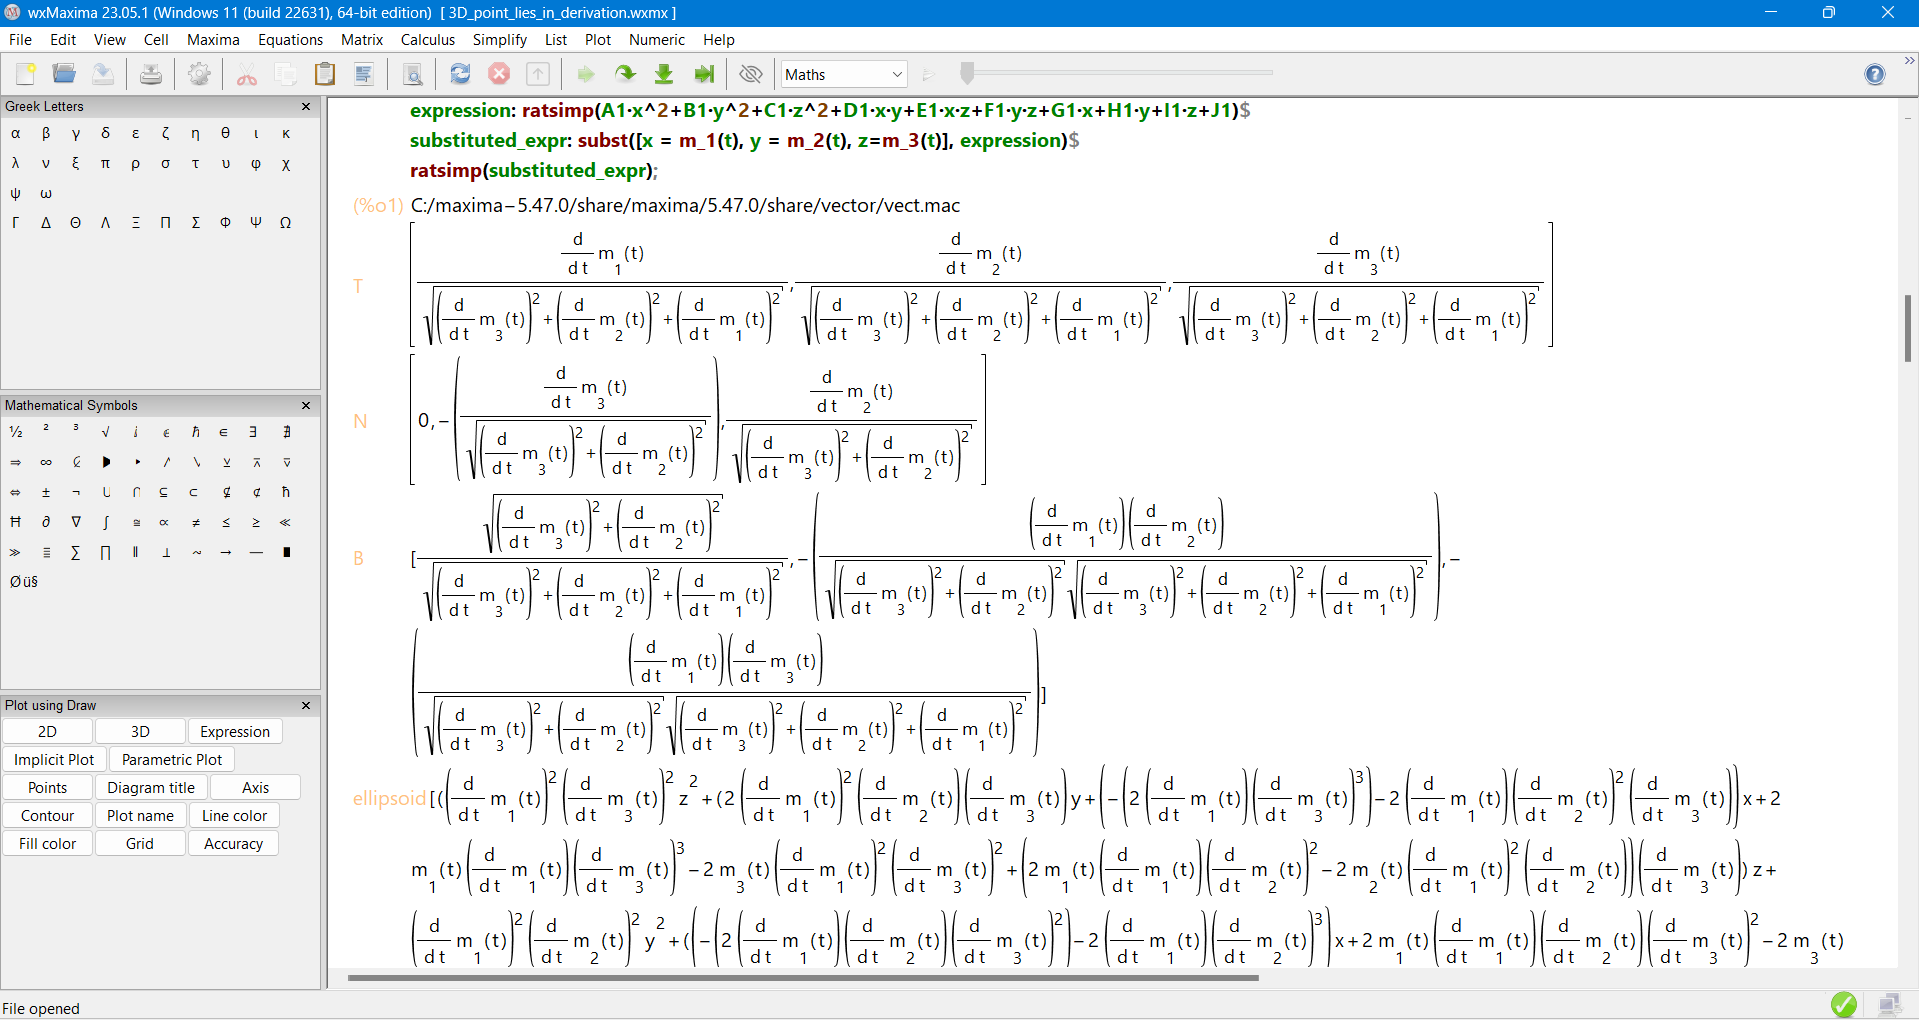
\includegraphics[width=\textwidth]{images/maxima.png}
	\caption[Softvér Maxima.]{Výpočet: bod v paramteri $t$ na krivke $m(t)$ leží v derivácii jednoparametrického systému elipsoidov.}
	\label{fig:3D_point_lies}
\end{figure}

